% Options for packages loaded elsewhere
\PassOptionsToPackage{unicode}{hyperref}
\PassOptionsToPackage{hyphens}{url}
%
\documentclass[
  12pt]{article}
\usepackage{amsmath,amssymb}
\usepackage{iftex}
\ifPDFTeX
  \usepackage[T1]{fontenc}
  \usepackage[utf8]{inputenc}
  \usepackage{textcomp} % provide euro and other symbols
\else % if luatex or xetex
  \usepackage{unicode-math} % this also loads fontspec
  \defaultfontfeatures{Scale=MatchLowercase}
  \defaultfontfeatures[\rmfamily]{Ligatures=TeX,Scale=1}
\fi
\usepackage{lmodern}
\ifPDFTeX\else
  % xetex/luatex font selection
\fi
% Use upquote if available, for straight quotes in verbatim environments
\IfFileExists{upquote.sty}{\usepackage{upquote}}{}
\IfFileExists{microtype.sty}{% use microtype if available
  \usepackage[]{microtype}
  \UseMicrotypeSet[protrusion]{basicmath} % disable protrusion for tt fonts
}{}
\makeatletter
\@ifundefined{KOMAClassName}{% if non-KOMA class
  \IfFileExists{parskip.sty}{%
    \usepackage{parskip}
  }{% else
    \setlength{\parindent}{0pt}
    \setlength{\parskip}{6pt plus 2pt minus 1pt}}
}{% if KOMA class
  \KOMAoptions{parskip=half}}
\makeatother
\usepackage{xcolor}
\usepackage{graphicx}
\makeatletter
\def\maxwidth{\ifdim\Gin@nat@width>\linewidth\linewidth\else\Gin@nat@width\fi}
\def\maxheight{\ifdim\Gin@nat@height>\textheight\textheight\else\Gin@nat@height\fi}
\makeatother
% Scale images if necessary, so that they will not overflow the page
% margins by default, and it is still possible to overwrite the defaults
% using explicit options in \includegraphics[width, height, ...]{}
\setkeys{Gin}{width=\maxwidth,height=\maxheight,keepaspectratio}
% Set default figure placement to htbp
\makeatletter
\def\fps@figure{htbp}
\makeatother
\setlength{\emergencystretch}{3em} % prevent overfull lines
\providecommand{\tightlist}{%
  \setlength{\itemsep}{0pt}\setlength{\parskip}{0pt}}
\setcounter{secnumdepth}{-\maxdimen} % remove section numbering
\usepackage{makeidx}
\makeindex
\usepackage{graphicx}
\usepackage{tikz}
\usepackage{atbegshi}
\AtBeginDocument{
	\AtBeginShipoutNext{
		\AtBeginShipoutUpperLeft{
			\put(\dimexpr\paperwidth/2-\textwidth/2\relax, -650){
				\makebox[\textwidth]{
\includegraphics[width=10cm]{logoMEDIA.jpeg}}
			}
		}
	}
}


\ifLuaTeX
  \usepackage{selnolig}  % disable illegal ligatures
\fi
\IfFileExists{bookmark.sty}{\usepackage{bookmark}}{\usepackage{hyperref}}
\IfFileExists{xurl.sty}{\usepackage{xurl}}{} % add URL line breaks if available
\urlstyle{same}
\hypersetup{
  pdftitle={Entrega: curso de datos extremales},
  pdfauthor={Laura Montaldo, CI: 3.512.962-7},
  hidelinks,
  pdfcreator={LaTeX via pandoc}}

\title{Entrega: curso de datos extremales}
\author{Laura Montaldo, CI: 3.512.962-7}
\date{2024-01-02}

\begin{document}
\maketitle

\newpage

\hypertarget{motivaciuxf3n-del-estudio}{%
\section{Motivación del estudio}\label{motivaciuxf3n-del-estudio}}

Se busca crear un indicador de una posible crisis bursátil. Como
variable de referencia de toma la relación de precios al cierre de ayer
sobre la de hoy \(Indicador=Precio_{t-1}/Precio_t\).

\vspace{1cm}

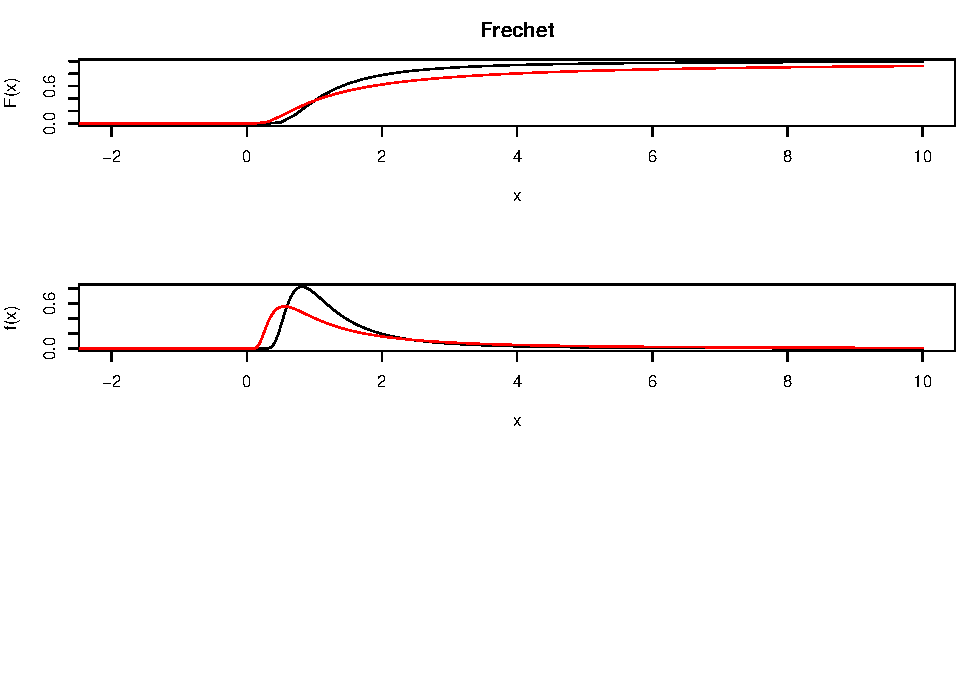
\includegraphics{extremales_files/figure-latex/unnamed-chunk-11-1.pdf}

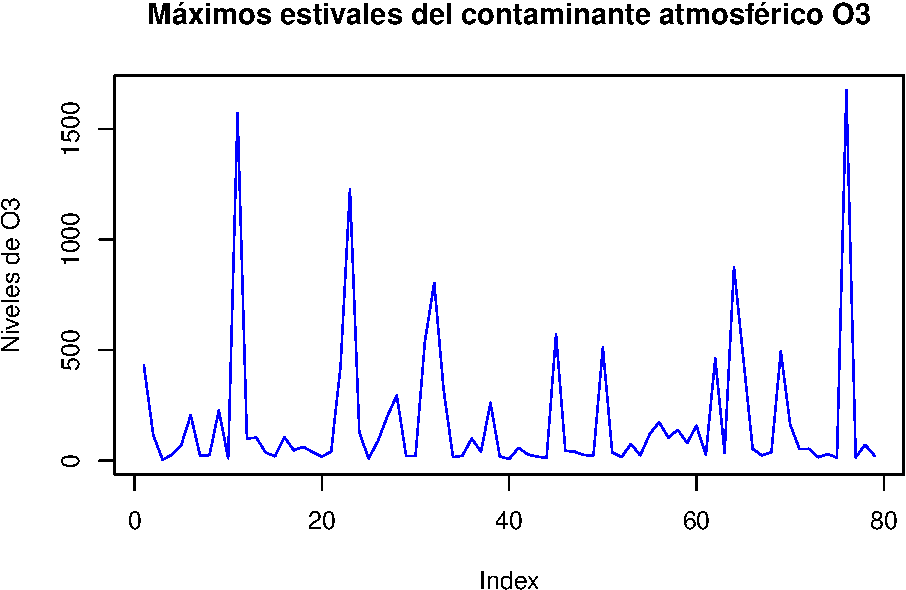
\includegraphics{extremales_files/figure-latex/unnamed-chunk-12-1.pdf}
\newpage

\hypertarget{marco-teuxf3rico}{%
\section{Marco Teórico}\label{marco-teuxf3rico}}

\hypertarget{teoruxeda-asintuxf3tica-cluxe1sica-y-las-distribuciones-extremales-y-sus-dominios-de-atracciuxf3n}{%
\subsection{Teoría asintótica clásica y las distribuciones extremales y
sus dominios de
atracción}\label{teoruxeda-asintuxf3tica-cluxe1sica-y-las-distribuciones-extremales-y-sus-dominios-de-atracciuxf3n}}

Siguiendo las notas del curso, se dice que tenemos datos extremos cuando
cada dato corresponde al máximo o mínimo de varios registros. Son un
caso particular de evento raro o gran desviación respecto a la media.

Asumiremos que nuestros datos son iid (independientes e idénticamente
distribuidos, son dos suposiciones juntas). Esta doble suposición suele
no ser realista en aplicaciones concretas ( ninguna de sus dos
componentes, incluso) pero para comenzar a entender la teoría clásica,
la utilizaremos por un tiempo.

Si tenemos datos \(X_1,...,X_n\) \(iid\) con distribución \(F\),
entonces \(X_n^* = max (X_1,...,X_n)\) tiene distribución \(F_n^*\) dada
por \(F_n^* (t)= F(t)_n\). Si conocemos la distribución \(F\)
conoceríamos la distribución \(F_n^*\) , pero en algunos casos la
lectura que queda registrada es la del dato máximo y no la de cada
observación que dio lugar al mismo, por lo que a veces ni siquiera es
viable estimar \(F\). Pero aún en los casos en que \(F\) es conocida o
estimable, si \(n\) es grande, la fórmula de \(F_n^*\) puede resultar
prácticamente inmanejable. En una línea de trabajo similar a la que
aporta el Teorema Central del Límite en la estadística de valores
medios, un teorema nos va a permitir aproximar \(F_n^*\) por
distribuciones más sencillas. Este es el Teorema de
Fischer-Tippet-Gnedenko (FTG, para abreviar) que presentaremos en breve.

Como \(X_1,...,X_n\) iid, definimos \(Y_i = -X_i\) para todo valor de
\(i\), entonces \(Y_1,...,Y_n\) iid y además
\(min(X_1,...,X_n) = - max(Y_1,...,Y_n)\) la teoría asintótica de los
mínimos de datos iid se reduce a la de los máximos, razón por la que nos
concentramos aquí en estudiar el comportamiento asintótico de los
máximos exclusivamente.

\hypertarget{las-distribuciones-extremales}{%
\subsection{Las distribuciones
extremales}\label{las-distribuciones-extremales}}

Las distribuciones extremales son tres: la distribución de Gumbel; la
distribución de Weibull; la distribución de Fréchet.

\hypertarget{distribuciuxf3n-de-gumbel}{%
\subsubsection{Distribución de Gumbel}\label{distribuciuxf3n-de-gumbel}}

Se dice que una variable tiene distribución de Gumbel si su distribución
es:

\[ \Lambda(x) = exp\{-e^{-x}\} \quad\text{para todo}\; x \;\text{real} \]

\hypertarget{distribuciuxf3n-de-weibull}{%
\subsubsection{Distribución de
Weibull}\label{distribuciuxf3n-de-weibull}}

Se dice que una variable tiene distribución de Weibull de orden
\(\alpha>0\) si su distribución es:

\[\Psi_{\alpha}(x)=\begin{cases}
exp{-(-x)^{\alpha}} & si\;x<0\\
1 & \text{en otro caso}
\end{cases}\]

\hypertarget{distribuciuxf3n-de-fruxe9chet}{%
\subsubsection{Distribución de
Fréchet}\label{distribuciuxf3n-de-fruxe9chet}}

Se dice que una variable tiene distribución de Fréchet de orden
\(\alpha>0\) si su distribución es:

\[
\Phi_{\alpha}(x)=\begin{cases}
exp\{-x^{-\alpha}\} & si\;x>0\\
0 & \text{en otro caso}
\end{cases}
\] \newpage

\hypertarget{teorema-1-relaciones-entre-las-versiones-standard-de-las-distribuciones-extremales.}{%
\subsubsection{Teorema 1: Relaciones entre las versiones standard de las
distribuciones
extremales.}\label{teorema-1-relaciones-entre-las-versiones-standard-de-las-distribuciones-extremales.}}

\(X\) tiene distribución \(\Phi_{\alpha}(x)\) si y sólo si \((-1/X)\)
tiene distribución \(\Psi_{\alpha}(x)\) si y sólo si \(log(X^{\alpha})\)
tiene distribución \(\Lambda\).

\end{document}
